%!TEX root = ../diss.tex
\tikzstyle{element}=[rectangle, thick,
                     inner sep=0.1cm, rounded corners]
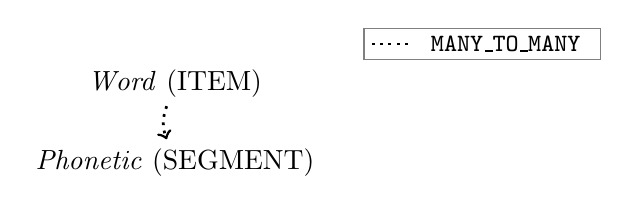
\begin{tikzpicture}

  \node (Word) at (0, 1) [element] {\textit{Word} (ITEM)};
  
  \node (Phonetic) at (0, 0) [element] {\textit{Phonetic} (SEGMENT)};

  \draw [->, line width=1, dotted] (Word) to [bend right=20] (Phonetic);

  %%%%%%%%%%%%%%%%%%%%%%%%%%%%%%
  % legends
  % simple
  \draw[gray] (2.4, 1.7) rectangle (5.4, 1.3);
  \node (leg_sim_m2m) at (4.2, 1.5) [element] {\small{\texttt{MANY\_TO\_MANY}}};
  \draw [-, line width=1, dotted] (2.5, 1.5) to (3.0, 1.5);

  
\end{tikzpicture}